% Created 2015-02-08 Sun 12:29
\documentclass[10pt]{article}
\usepackage[utf8]{inputenc}
\usepackage[T1]{fontenc}
\usepackage[letterpaper]{geometry}
\geometry{verbose,tmargin=1.5cm,bmargin=1.5cm,lmargin=1.5cm,rmargin=1.5cm,columnsep=0.8cm}
\usepackage[english]{babel}
\usepackage{graphicx}
\usepackage{longtable}
\usepackage{float}
\usepackage{fouriernc}
\usepackage{amssymb}
\usepackage{hyperref}
\usepackage{framed}
\tolerance=1000
\providecommand{\alert}[1]{\textbf{#1}}
\usepackage{enumitem}
\usepackage{multicol}

\usepackage{tikz}
\usetikzlibrary{arrows,automata,positioning,fit,shapes}
 
\begin{document}

\begin{center}
\huge EECE7398 --- Compilers

Assignment 4

\vskip1cm

\normalsize\ttfamily Bruno S M M Morais <soutomaiormunizmo.b@husky.neu.edu>

%All code can be found on \url{https://bitbucket.org/brunosmmm/eece7352code_public}

\end{center}

\vskip1cm

\section*{Question 1}
\subsection*{item (a)}

\large

The following substitutions are made:

\begin{enumerate}
\item $(\bullet)+ \Rightarrow (\bullet)(\bullet)*$
\item $(\bullet)? \Rightarrow (\bullet | \varepsilon)$
\end{enumerate}

Yielding:

$\left( +|-| \varepsilon \right) [0-9][0-9]* ((.[0-9][0-9]*)|\varepsilon)$

\subsection*{item (b)}

\begin{figure}[H]
\centering

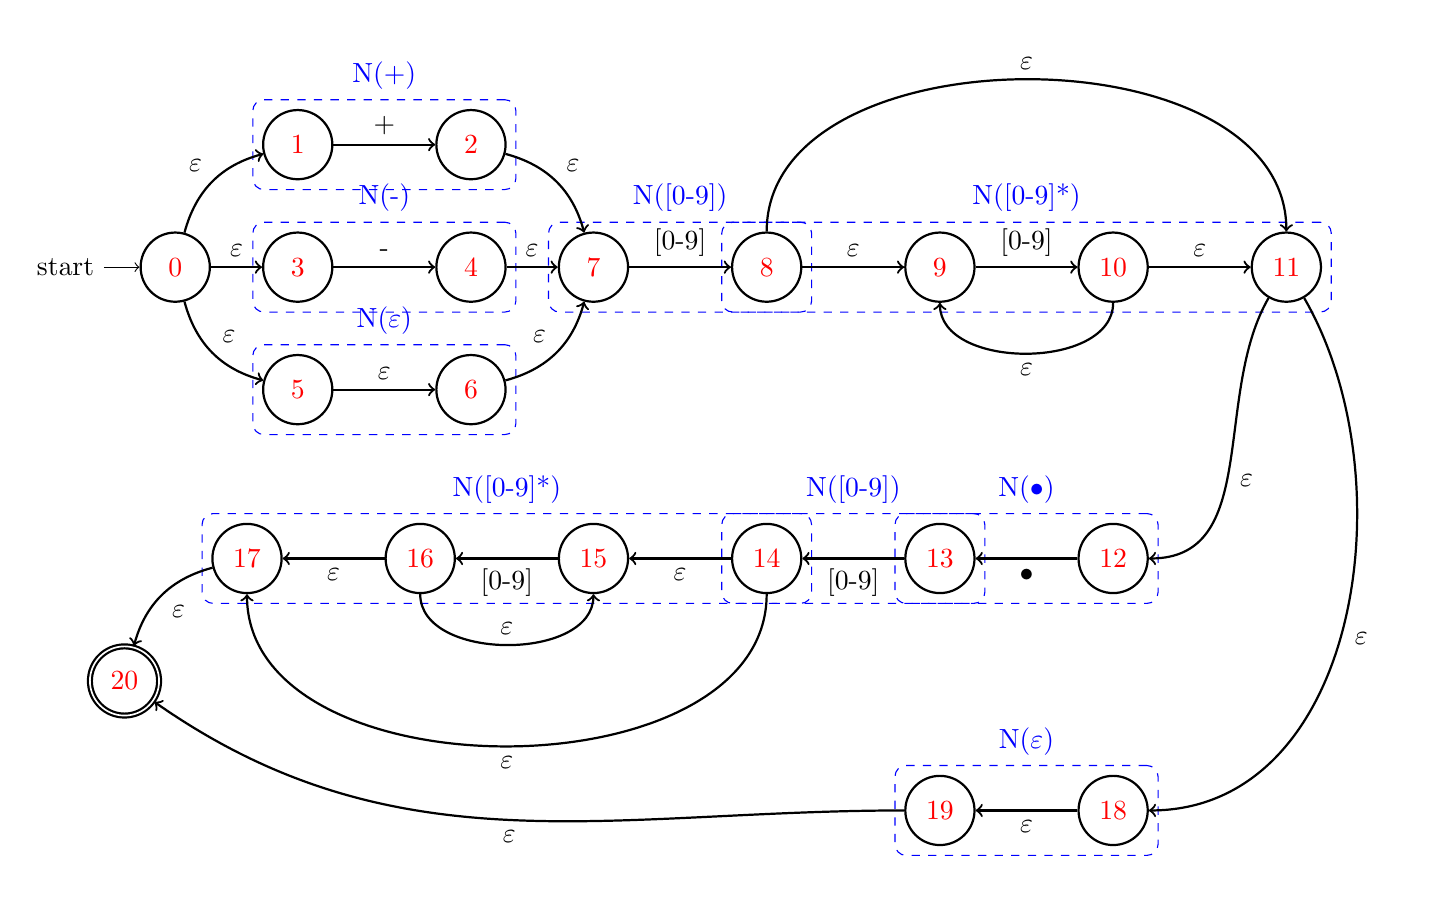
\begin{tikzpicture}[auto,node distance = 2.2cm]

\tikzstyle{every state}=[thick,fill=none,draw=black,text=red]
\tikzstyle{nfabound}=[draw=blue,rounded corners,dashed]

%(+|-|epsilon)[0-9][0-9]*((.[0-9][0-9]*)|epsilon)

\node[initial,state] (s0) {0};

%+
\node[state]         (s1) [above right of=s0] {1};
\node[state]         (s2) [right of=s1] {2};

\node[nfabound,fit= (s1) (s2),label={[blue]N(+)}] {};

%-
\node[state]         (s3) at (s1 |- s0) {3};
\node[state]         (s4) [right of=s3] {4};

\node[nfabound,fit= (s3) (s4),label={[blue]N(-)}] {};

%Epsilon
\node[state]         (s5) [below right of=s0] {5};
\node[state]         (s6) [right of=s5]       {6};

\node[nfabound,fit= (s5) (s6),label={[blue]N($\varepsilon$)}] {};

%get out of first nfa
\node[state]         (s7) [below right of=s2]       {7};

%(+|-|epsilon) bounding box
%\node[nfabound,fit=(s0) (s1) (s2) (s3) (s4) (s5) (s6) (s7),label={[blue]N($\left( + | - | \varepsilon \right)$}] {};

%second part of regex -> [0-9]
\node[state]         (s8) [right of=s7] {8};
\node[nfabound,fit=(s7) (s8),label={[blue]N([0-9])}] {};
%next -> [0-9]*
\node [state]        (s9) [right of=s8] {9};
\node [state]        (s10) [right of=s9] {10};
\node [state]        (s11) [right of=s10] {11};
\node[nfabound,fit=(s8) (s9) (s10) (s11),label={[blue]N([0-9]*)}] {};

%next
\node [state]        (s12) [below of=s10,yshift=-1.5cm] {12};
\node [state]        (s13) [left of=s12] {13};
\node [state]        (s14) [left of=s13] {14};

\node[nfabound,fit=(s12) (s13),label={[blue]N($\bullet$)}] {};
\node[nfabound,fit=(s13) (s14),label={[blue]N([0-9])}] {};

\node [state]        (s15) [left of=s14] {15};
\node [state]        (s16) [left of=s15] {16};
\node [state]        (s17) [left of=s16] {17};
\node[nfabound,fit=(s14) (s15) (s16) (s17),label={[blue]N([0-9]*)}] {};

%empty
\node [state]        (s18) [below of=s12, yshift=-1cm] {18};
\node [state]        (s19) [left of=s18] {19};

\node[nfabound,fit=(s18) (s19),label={[blue]N($\varepsilon$)}] {};

%final state
\node [state,accepting]        (f) [below left of=s17] {20};

%first to + nfa
\path [->,thick] (s0) edge [bend left] node {$\varepsilon$} (s1)
      [->,thick] (s1) edge node {+} (s2)
      [->,thick] (s2) edge [bend left] node {$\varepsilon$} (s7)
%now to - nfa
      [->,thick] (s0) edge node {$\varepsilon$} (s3)
      [->,thick] (s3) edge node {-} (s4)
      [->,thick] (s4) edge node {$\varepsilon$} (s7)
%empty NFA
      [->,thick] (s0) edge [bend right] node {$\varepsilon$}  (s5)
      [->,thick] (s5) edge node {$\varepsilon$}  (s6)
      [->,thick] (s6) edge [bend right] node {$\varepsilon$}  (s7)
%to next part
      [->,thick] (s7) edge node {[0-9]} (s8)
%next
      [->,thick] (s8) edge node {$\varepsilon$} (s9)
      [->,thick] (s9) edge node {[0-9]} (s10)
      [->,thick] (s10) edge node {$\varepsilon$} (s11)
      [->,thick] (s10) edge [out=270,in=270] node {$\varepsilon$} (s9)
      [->,thick] (s8)  edge [out=90,in=90] node {$\varepsilon$} (s11)
%next
      [->,thick] (s11) edge [out=240,in=0] node {$\varepsilon$} (s12)
      [->,thick] (s12) edge node {$\bullet$} (s13) 
      [->,thick] (s13) edge node {[0-9]} (s14)
      [->,thick] (s14) edge node {$\varepsilon$} (s15)
      [->,thick] (s15) edge node {[0-9]} (s16)
      [->,thick] (s16) edge node {$\varepsilon$} (s17)
      [->,thick] (s14) edge [out=270,in=270] node {$\varepsilon$} (s17)
      [->,thick] (s16) edge [out=270,in=270] node {$\varepsilon$} (s15)
%empty
      [->,thick] (s11) edge [out=300,in=0] node {$\varepsilon$} (s18)
      [->,thick] (s18) edge node {$\varepsilon$} (s19)
%final state
      [->,thick] (s17) edge [bend right] node {$\varepsilon$} (f)
      [->,thick] (s19) edge [out=180,in=325] node {$\varepsilon$} (f);

\end{tikzpicture}
\caption{NFA for regular expression on item (a)}
\end{figure}

\subsection*{item (c)}

Files for this item are attached to blackboard submission.

\pagebreak

\section*{Question 2}

\subsection*{item (a)}

First we need to specify all the tokens types that need to be recognized:

\begin{table}[H]
\centering
\begin{tabular}{p{4cm} l}
\bfseries Lexeme & \bfseries Token \\
\hline
My\_2nd\_var     & <ID, ``My\_2nd\_var''> \\
=                & <assign> \\
2                & <number, 2> \\
;                & <semicolon> \\
if               & <if>        \\
(                & <open\_par> \\
x                & <ID, ``x''> \\
)                & <close\_par> \\
return           & <return>  \\
a                & <ID, ``a''> \\
==               & <isequal>  \\
1                & <number, 1> \\
;                & <semicolon> \\
\hline
\end{tabular}
\caption{Lexemes in code snippet}
\end{table}

Note that for this exercise, spaces (newlines, tabs and single spaces) are considered also lexemes, and will be printed out by the scanner program.

\begin{table}[H]
\centering
\begin{tabular}{p{4cm} l}
\bfseries Regular definition & \bfseries Regular Expression\\
\hline
number     &   [0-9]+ \\
ID         &   [a-zA-Z\_][a-zA-Z0-9\_]+ \\
assign     &   = \\
semicolon  &   ; \\
open\_par  &   ``('' \\
close\_par &   ``)'' \\
isequal    &   == \\
return     &   return \\
if         &   if \\
space      &   [\textbackslash n\textbackslash t\textvisiblespace]+ \\
\hline
\end{tabular}
\caption{Regular definitions and expressions for scanning}
\end{table}


\begin{figure}[H]
\centering
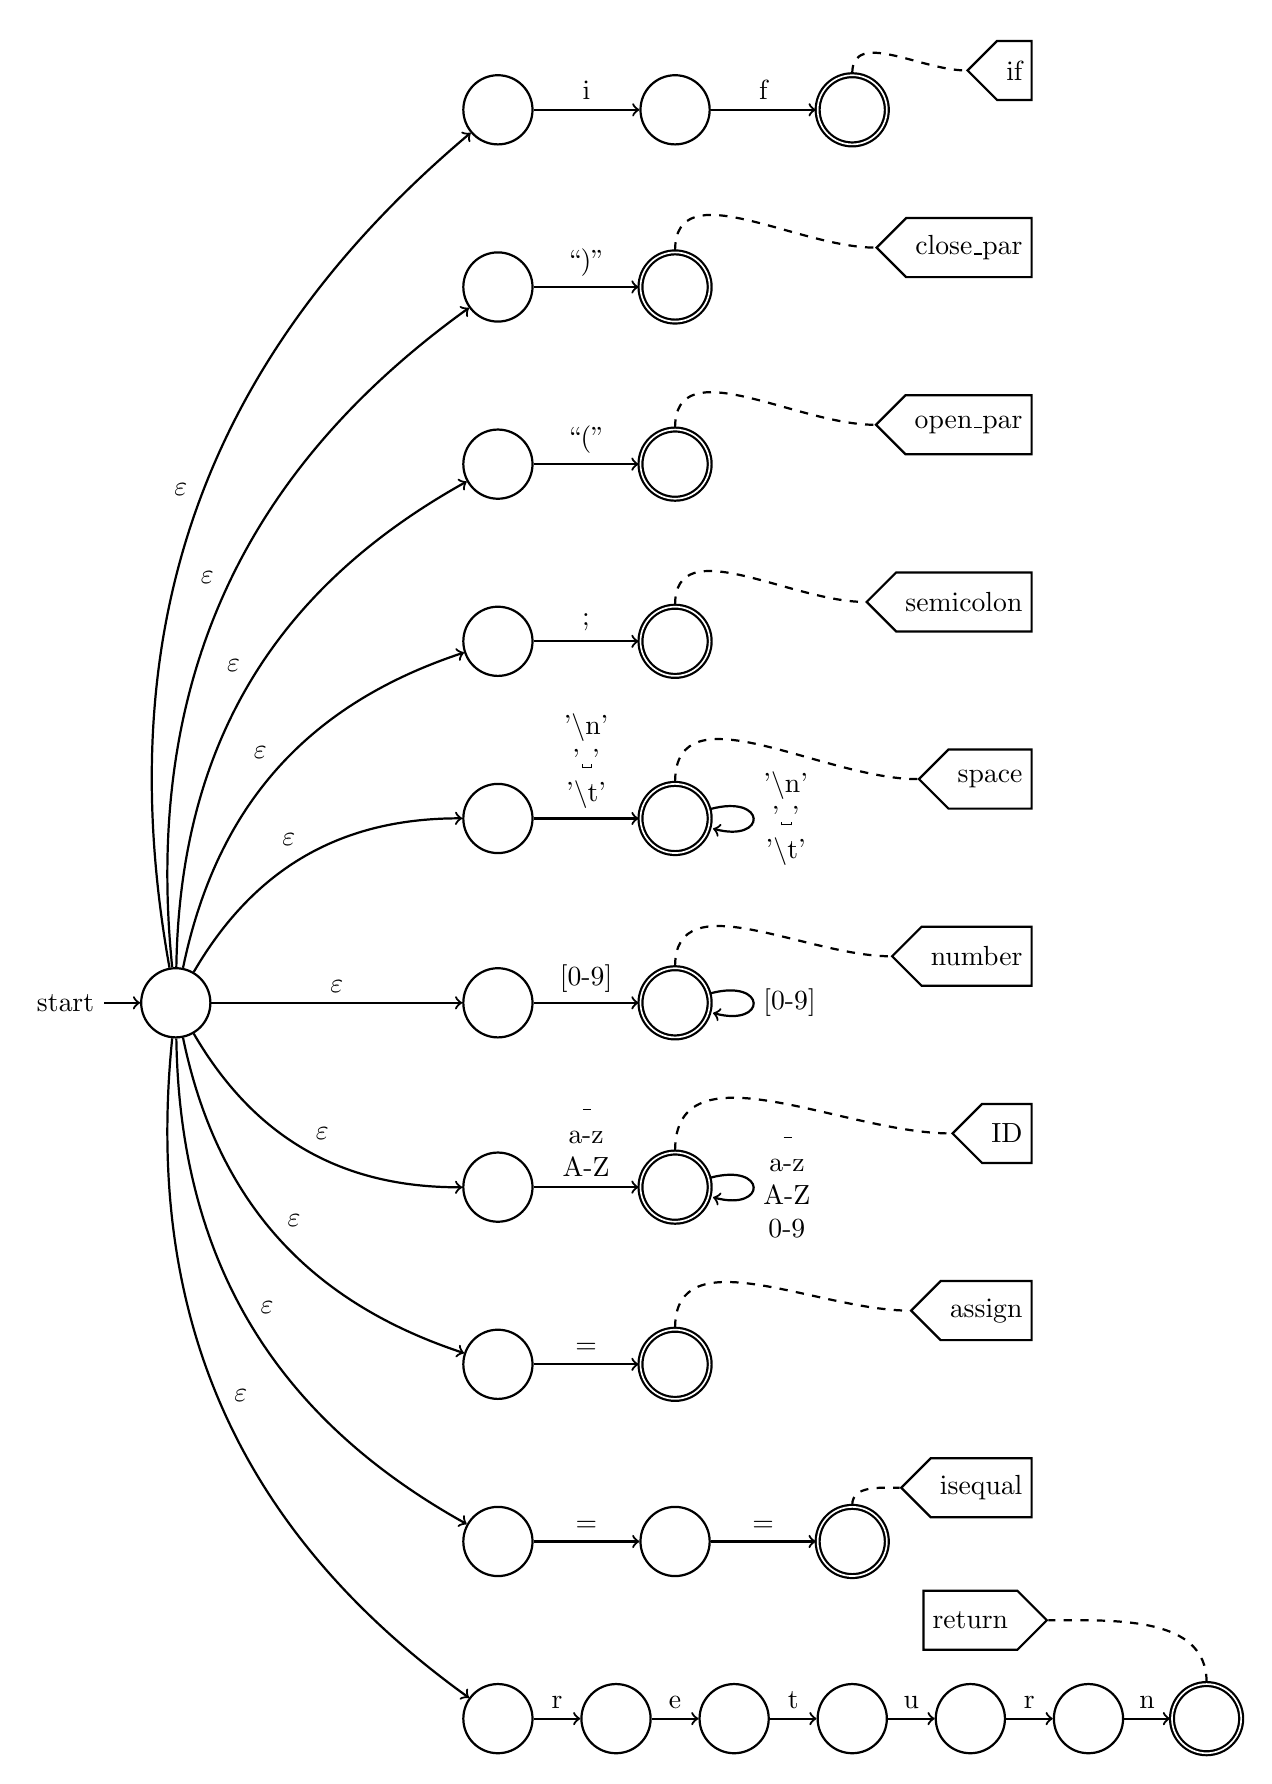
\begin{tikzpicture}[->,thick,auto,node distance = 2.25cm]

\tikzstyle{every state}=[thick,fill=none,draw=black,text=red]

%initial state
\node [initial,state] (s) {};

%NFA for spaces
\node [state] (space0) [above right of=s,yshift=0.75cm,xshift=2.5cm] {};
\node [state,accepting] (spacef) [right of=space0] {};

\node [draw=black,signal,signal to=west,node distance=4cm,minimum size=0.75cm] (spacet) [right of=spacef,yshift=0.5cm] {space};

\path (s) edge [bend left] node {$\varepsilon$} (space0)
      (space0) edge node[align=center] {'\textbackslash n'\\'\textvisiblespace'\\'\textbackslash t'} (spacef)
      (spacef) edge [loop right] node[align=center] {'\textbackslash n'\\'\textvisiblespace'\\'\textbackslash t'} ();

\path  [-,dashed] (spacef) edge [out=90,in=180] (spacet);

%NFA for numbers
\node [state] (num0) at (space0 |- s) {};
\node [state,accepting] (numf) [right of=num0] {};

\node [draw=black,signal,signal to=west,minimum size=0.75cm] (numt) [below= of spacet.east,anchor=east] {number};

\path (s) edge node {$\varepsilon$} (num0)
      (num0) edge node[align=center] {[0-9]} (numf)
      (numf) edge [loop right] node {[0-9]} ();

\path  [-,dashed] (numf) edge [out=90,in=180] (numt);

%NFA for identifiers
\node [state] (id0) [below right of=s,yshift=-0.75cm,xshift=2.5cm] {};
\node [state,accepting] (idf) [right of=id0] {};

\node [draw=black,signal,signal to=west,minimum size=0.75cm] (idt) [below= of numt.east,anchor=east] {ID};

\path (s) edge [bend right] node {$\varepsilon$} (id0)
      (id0) edge node[align=center] {\_\\a-z\\A-Z} (idf)
      (idf) edge [loop right] node[align=center] {\_\\a-z\\A-Z\\0-9} ();

\path  [-,dashed] (idf) edge [out=90,in=180] (idt);

%%NFAs for reserved words and operators
%assign
\node [state] (eq0) [below of=id0] {};
\node [state,accepting] (eqf) [right of=eq0] {};

\node [draw=black,signal,signal to=west,minimum size=0.75cm] (eqt) [below= of idt.east,anchor=east] {assign};

\path (s) edge [bend right] node {$\varepsilon$} (eq0)
      (eq0) edge node {=} (eqf);

\path  [-,dashed] (eqf) edge [out=90,in=180] (eqt);

%equal
\node [state] (iseq0) [below of=eq0] {};
\node [state] (iseq1) [right of=iseq0] {};
\node [state,accepting] (iseqf) [right of=iseq1] {};

\node [draw=black,signal,signal to=west,minimum size=0.75cm] (iseqt) [below= of eqt.east,anchor=east] {isequal};

\path (s) edge [bend right] node {$\varepsilon$} (iseq0)
      (iseq0) edge node {=} (iseq1)
      (iseq1) edge node {=} (iseqf);

\path  [-,dashed] (iseqf) edge [out=90,in=180] (iseqt);

%semicolon
\node[state] (sc0) [above of=space0] {};
\node[state,accepting] (scf) [right of=sc0] {};

\node [draw=black,signal,signal to=west,minimum size=0.75cm] (sct) [above= of spacet.east,anchor=east] {semicolon};

\path (s) edge [bend left] node {$\varepsilon$} (sc0)
      (sc0) edge node {;} (scf);

\path  [-,dashed] (scf) edge [out=90,in=180] (sct);

%open parenthesis
\node[state] (opar0) [above of=sc0] {};
\node[state,accepting] (oparf) [right of=opar0] {};

\node [draw=black,signal,signal to=west,minimum size=0.75cm] (opart) [above= of sct.east,anchor=east] {open\_par};

\path (s) edge [bend left] node {$\varepsilon$} (opar0)
      (opar0) edge node {``(''} (oparf);

\path  [-,dashed] (oparf) edge [out=90,in=180] (opart);

%close parenthesis
\node[state] (cpar0) [above of=opar0] {};
\node[state,accepting] (cparf) [right of=cpar0] {};

\node [draw=black,signal,signal to=west,minimum size=0.75cm] (cpart) [above =of opart.east,anchor=east] {close\_par};

\path (s) edge [bend left] node {$\varepsilon$} (cpar0)
      (cpar0) edge node {``)''} (cparf);

\path  [-,dashed] (cparf) edge [out=90,in=180] (cpart);

%return
\node [state] (ret0) [below of=iseq0] {};
\node [state,node distance=1.5cm] (ret1) [right of=ret0] {};
\node [state,node distance=1.5cm] (ret2) [right of=ret1] {};
\node [state,node distance=1.5cm] (ret3) [right of=ret2] {};
\node [state,node distance=1.5cm] (ret4) [right of=ret3] {};
\node [state,node distance=1.5cm] (ret5) [right of=ret4] {};
\node [state,accepting,node distance=1.5cm] (retf) [right of=ret5] {};

\node [draw=black,signal,signal to=east,minimum size=0.75cm] (rett) [above of=ret4,yshift=-1cm] {return};

\path (s) edge [bend right] node {$\varepsilon$} (ret0)
      (ret0) edge node {r} (ret1)
      (ret1) edge node {e} (ret2)
      (ret2) edge node {t} (ret3)
      (ret3) edge node {u} (ret4)
      (ret4) edge node {r} (ret5)
      (ret5) edge node {n} (retf);   

\path  [-,dashed] (retf) edge [out=90,in=0] (rett);

%if
\node [state] (if0) [above of=cpar0] {};
\node [state] (if1) [right of=if0] {};
\node [state,accepting] (iff) [right of=if1] {};

\node [draw=black,signal,signal to=west,minimum size=0.75cm,align=right] (ift) [above= of cpart.east,anchor=east] {if};

\path (s) edge [bend left] node {$\varepsilon$} (if0)
      (if0) edge node {i} (if1)
      (if1) edge node {f} (iff); 

\path  [-,dashed] (iff) edge [out=90,in=180] (ift);

\end{tikzpicture}
\caption{Scanner NFA}
\end{figure}

\subsection*{item (b)}

Source code uploaded to blackboard.

\end{document}
